\chapter{Event Building}
\label{ch:events}

\corry implements a very flexible algorithm for offline event building that allows data to be combined from devices with different readout schemes.
This is possible via the concept of detector modules, which allows data to be processed from different detectors individually as described in Section~\ref{sec:module_manager}.
Events are processed sequentially as described in Chapter~\ref{ch:framework}.

The following sections provide an introduction to event building and detail the procedure using a few examples.

\section{The Order of the Event Loaders is Key}

When building events, it is important to carefully choose the order of the event loader modules.
An event loader module is defined as a module which reads an external data source and places \corry objects on the clipboard.
The first module to be run has to define the extent of the event by defining the \parameter{Event} object on the clipboard either through trigger numbers or a time window.

Apart from modules named \module{EventLoader<...>}, also the \module{Metronome} and \module{FileReader} modules are considered event loader modules since they read external data sources and/or define the clipboard \parameter{Event} object.

\begin{warning}
Once this event is set, no changes to its start and end time are possible, and no new event definition can be set by a subsequent module.
\end{warning}

Following modules in the reconstruction chain can only access the defined event and compare its extent in time or assigned trigger IDs to the currently processed data.
A special case are triggered devices that do not provide reference timestamps, as will be discussed in Section~\ref{sec:triggered_devices}.
The event is cleared at the end of the processing chain.

However, not all event loader modules are capable of defining an event.
Detectors that run in a data-driven mode usually just provide individual measurements together with a time stamp.
In order to slice this continuous data stream into consumable frames, the \module{Metronome} module can be used as described in Section~\ref{sec:metronome}.

The order of event loader modules can be explicitly specified by using multiple instances and assigning them to individual detectors as described in Section~\ref{sec:module_instantiation}:

\begin{minted}[frame=single,framesep=3pt,breaklines=true,tabsize=2,linenos]{ini}
# First process data from the detector named "CP01_W03"
[EventLoaderEUDAQ2]
name = "CP01_W03"

# Now process all detectors of type "Timepix3"
[EventLoaderEUDAQ2]
type = "Timepix3"

# Finally, process all remaining detectors in order along the z-axis
[EventLoaderEUDAQ2]
\end{minted}

Otherwise, the order in which the detectors are placed along the z-axis in the geometry is used.

\subsection{Position of Event Data: Before, During, or After?}

After the event has been defined, subsequent modules should compare their currently processed data to the defined event.
For this, the event object can be retrieved from the clipboard storage and the event data of the current detector can be tested against it using a set of member functions.
These functions return one of the following four possible positions:
\begin{description}
        \item[\textbf{\parameter{BEFORE}:}] The data currently under consideration are dated \emph{before} the event. Therefore they should be discarded and more data should be processed.
        \item[\textbf{\parameter{DURING}:}] The data currently under consideration are \emph{within} the defined event frame and should be taken into account. More data should be processed.
        \item[\textbf{\parameter{UNDEFINED}:}] The data currently under consideration are \emph{within} the defined event but does not belong to it. The data should be skipped and the next data should be processed until one of the other conditions is met.
        \item[\textbf{\parameter{AFTER}:}] The data are dated \emph{after} the current event has finished. The processing of data for this detector should therefore be stopped and the current data retained for consideration in the next event.
        \item[\textbf{\parameter{UNKNOWN}:}] The event does not allow the position in time of the data to be determined. The data should be skipped and the next data should be processed until one of the above conditions can be reached.
\end{description}

Depending on what information is available from detector data, different member functions are available.

\subsection{Data-Driven Detectors}
If the data provides a single timestamp, such as the data from a data-driven detector, the \command{getTimestampPosition()} function can be used:

\begin{minted}[frame=single,framesep=3pt,breaklines=true,tabsize=2,linenos]{c++}
// Timestamp of the data currently under scrutiny:
double my_timestamp = 1234;
// Fetching the event definition
auto event = clipboard->getEvent();
// Comparison of the timestamp to the event:
auto position = event->getTimestampPosition(my_timestamp);
\end{minted}

Since an event \emph{always} has to define its beginning and end, this function cannot return an \parameter{UNKNOWN} position.

\subsection{Frame-Based Detectors}
If the data to be added are from a source that defines a time frame, such as frame-based or shutter-based detectors, there are two timestamps to consider.
The appropriate function for position comparison is called \command{getFramePosition()} and takes two timestamps for beginning and end of the data frame, as well as an additional flag to choose between the interpretation modes \emph{inclusive} and \emph{exclusive} (see below).
Several modules, such as the \command{EventLoaderEUDAQ2}, employ a configuration parameter to influence the matching behavior.

\paragraph{Inclusive Selection:}
The inclusive interpretation will return \parameter{DURING} as soon as there is some overlap between the frame and the event, i.e. as soon as the end of the frame is later than the event start or the frame start is before the event end.

If the event has been defined by a reference detector, this mode can be used for the DUT to make sure the data extends well beyond the devices providing the reference tracks.
This allows for the correct measurement of e.g.\ the efficiency without being biased by DUT data that lies outside the frame of the reference detector.

\paragraph{Exclusive Selection:}
In the exclusive mode, the frame will be classified as \parameter{DURING} only if the start and end are both within the defined event.
This mode could be used if the event is defined by the DUT itself.
In this case the reference data that is added to the event should not extend beyond this boundary but should only be considered if it is fully contained within the DUT event to avoid the creation of artificial inefficiencies.

The \command{getFramePosition()} takes the start and end times as well as the matching behavior flag:

\begin{minted}[frame=single,framesep=3pt,breaklines=true,tabsize=2,linenos]{c++}
// Timestamp of the data currently under scrutiny:
double my_frame_start = 1234, my_frame_stop = 1289;
// Fetching the event definition
auto event = clipboard->getEvent();
// Comparison of the frame to the event, in this case inclusive:
auto position = event->getFramePosition(my_frame_start, my_frame_stop, true);
\end{minted}

The function returns \parameter{UNKNOWN} if the end of the given time frame is before its start and therefore ill-defined.

\subsection{Triggered Devices Without Timestamp}
\label{sec:triggered_devices}

Many devices return data on the basis of external trigger decisions.
If the device also provides a timestamp, the data can be directly assigned to events based on the algorithms outlined above.

The situation becomes more problematic if the respective data only have the trigger ID or number assigned but should be combined with un-triggered devices that define their events based on timestamps only.

In order to process such data, a device which relates timestamps and trigger IDs such as a trigger logic unit, is required.
This device should be placed before the detector in question in order to assign trigger IDs to the event using the \command{addTrigger(...)} function.
Then, the triggered device without timestamps can query the event for the position of its trigger ID with respect to the event using \command{getTriggerPosition()}:

\begin{minted}[frame=single,framesep=3pt,breaklines=true,tabsize=2,linenos]{c++}
// Trigger ID of the current data
uint32_t my_trigger_id = 1234;
// Fetching the event definition
auto event = clipboard->getEvent();
// Comparison of the trigger ID to the event
auto position = event->getTriggerPosition(my_trigger_id);
\end{minted}

If the given trigger ID is smaller than the smallest trigger ID known to the event, the function places the data as \parameter{BEFORE}.
If the trigger ID is larger than the largest know ID, the function returns \parameter{AFTER}. If the trigger ID is known to the event, the respective data is dated as being \parameter{DURING} the current event.
In cases where either no trigger ID has been previously added to the event or where the given ID lies between the smallest and largest known ID but is not part of the event, \parameter{UNKNOWN} is returned.

\section{The Metronome}
\label{sec:metronome}

In some cases, none of the available devices require a strict event definition such as a trigger or a frame.
This is sometimes the case when all or many of the involved devices have a data-driven readout.

\begin{figure}[tbp]
        \centering
        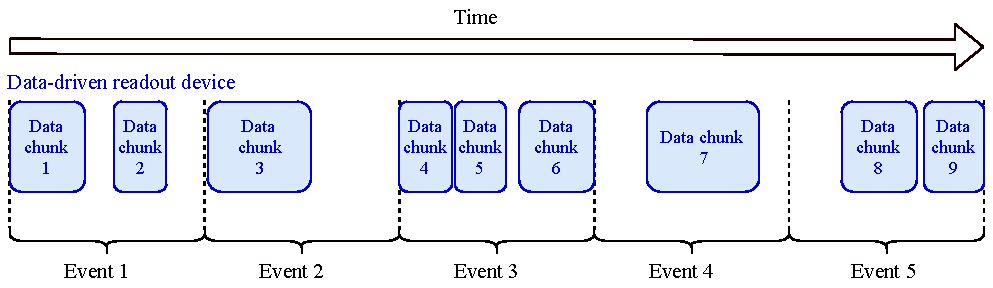
\includegraphics[width=1.0\textwidth]{corrymanual_eventbuilding_datadriven.pdf}
        \caption{Event building with fixed-length time frames from the Metronome for data-driven detectors}
        \label{fig:datadriven}
\end{figure}

In this situation, the \module{Metronome} module can be used to slice the data stream into regular time frames with a defined length, as indicated in Figure~\ref{fig:datadriven}.

In addition to splitting the data stream into frames, trigger numbers can be added to each of the frames as described in the module documentation of the \module{Metronome} in Section~\ref{metronome}.
This can be used to process data exclusively recorded with triggered devices, where no timing information is available or necessary from any of the devices involved.
The module should then be set up to always add one trigger to each of its events, and all subsequent detectors will simply compare to this trigger number and add their event data.

If used, the \module{Metronome} module always has to be placed as first module in the data analysis chain because it will attempt to define the event and to add it to the clipboard.
This operation fails if an event has already been defined by a previous module.


\section{Example Configurations for Event Building}

In these examples, it is assumed that all data have been recorded using the \emph{EUDAQ2} framework, and that the \module{EventLoaderEUDAQ2} is used for all devices to read and decode their data.
+However, this example pattern is not limited to that case and a very similar configuration could be used when the device data have been stored into device-specific native data files.

\subsection{Event Definition by Frame-Based DUT}
\label{sec:reco_mixedmode}
\begin{figure}[tbp]
        \centering
        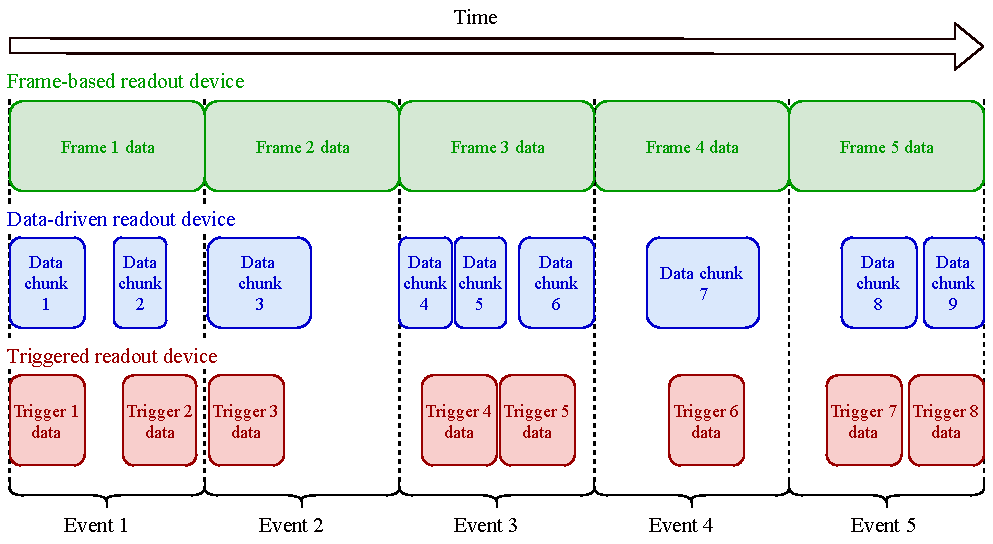
\includegraphics[width=1.0\textwidth]{corrymanual_eventbuilding_framebased.pdf}
        \caption{Event building strategy in a mixed-mode situation with devices adhering to different readout schemes. Here, the event is defined by the frame-based device and all other data are added within the event boundaries.}
        \label{fig:datadrivenandframebased}
\end{figure}

This example demonstrates the setup for event building based on a frame-based DUT.
The event building strategy for this situation is sketched in Figure~\ref{fig:datadrivenandframebased}.
The configuration contains four different devices:
\begin{description}
        \item[\parameter{CLICpix2}~\cite{clicpix2}:] This prototype acts as device under test and is a detector designed for operation at a linear collider, implementing a frame-based readout scheme. In this example, it will define the event.
        \item[\parameter{TLU}~\cite{aida-tlu}:] The trigger logic unit records scintillator coincidence signals with their respective timestamps, generates trigger signals and provides the reference clock for all other devices.
        \item[\parameter{Timepix3}~\cite{timepix3}:] This detector is operated in its data-driven mode, where the external clock from the TLU is used to timestamp each individual pixel hit. The hits are directly read out and sent to the data acquisition system in a continuous data stream.
        \item[\parameter{MIMOSA26}~\cite{mimosa26}:] These detectors are devices with a continuous rolling shutter readout, which do not record any timing information in the individual frames. The data are tagged with the incoming trigger IDs by its DAQ system.
\end{description}

In order to build proper events from these devices, the following configuration is used:

\begin{minted}[frame=single,framesep=3pt,breaklines=true,tabsize=2,linenos]{ini}
[Corryvreckan]
# ...

[EventLoaderEUDAQ2]
name = "CLICpix2_0"
file_name = /data/run001_file_caribou.raw

[EventLoaderEUDAQ2]
name = "TLU_0"
file_name = /data/run001_file_ni.raw

[EventLoaderEUDAQ2]
name = "Timepix3_0"
file_name = /data/run001_file_spidr.raw

[EventLoaderEUDAQ2]
type = "MIMOSA26"
file_name = /data/run001_file_ni.raw
\end{minted}

The first module will define the event using the frame start and end timestamps from the \parameter{CLICpix2} device.
Then, the data from the \parameter{TLU} are added by comparing the trigger timestamps to the event.
The matching trigger numbers are added to the event for later use.
Subsequently, the \parameter{Timepix3} device adds its data to the event by comparing the individual pixel timestamps to the existing event definition.
Finally, the six \parameter{MIMOSA26} detectors are added one-by-one via the automatic \parameter{type}-instantiation of detector modules described in Section~\ref{sec:module_instantiation}.
Here, the trigger numbers from the detector data are compared to the ones stored in the event as described in Section~\ref{sec:triggered_devices}.

It should be noted that in this example, the data from the \parameter{TLU} and the six \parameter{MIMOSA26} planes are read from the same file.
The event building algorithm is transparent to how the individual detector data are stored, and the very same building pattern could be used when storing the data in separate files.
In addition, it should be noted that swapping the order of the \parameter{Timepix3} and \parameter{MIMOSA26} detectors is also a valid configuration with identical results to the above scheme.

\subsection{Event Definition by Trigger Logic Unit}
This example demonstrates the setup for event building based on the trigger logic unit.
The configuration contains the same devices as the example in Section~\ref{sec:reco_mixedmode} but replaces the \parameter{CLICpix2} by the \parameter{ATLASpix}:
\begin{description}
        \item[\parameter{ATLASpix}~\cite{atlaspix}:] This prototype acts as device under test and is a detector initially designed for the ATLAS ITk upgrade, implementing a triggerless column-drain readout scheme.
\end{description}

In order to build proper events from these devices, the following configuration is used:

\begin{minted}[frame=single,framesep=3pt,breaklines=true,tabsize=2,linenos]{ini}
[Corryvreckan]
# ...

[EventLoaderEUDAQ2]
name = "TLU_0"
file_name = /data/run001_file_ni.raw
adjust_event_times = [["TluRawDataEvent", -115us, +230us]]

[EventLoaderEUDAQ2]
type = "MIMOSA26"
file_name = /data/run001_file_ni.raw

[EventLoaderEUDAQ2]
name = "Timepix3_0"
file_name = /data/run001_file_spidr.raw

[EventLoaderALTASpix]
name = "ATLASpix_0"
input_directory = /data/run001/
\end{minted}

The first module will define the event using the frame start and end timestamps from the \parameter{TLU} device.
As in the previous example, the \parameter{MIMOSA26} data will be added based on the trigger number.
The frame start provided by the \parameter{TLU} corresponds to the trigger timestamp and the frame end is one clockcycle later.
However, due to the rolling shutter readout scheme, the hits that are read out from the \parameter{MIMOSA26} planes when receiving a trigger may have happened in a time period before or after the trigger signal.
Consequently, the event times need to be corrected using the \parameter{adjust_event_times} parameter (described in Section~\ref{eventloadereudaq2}) such that the data from the \parameter{ATLASpix} and \parameter{Timepix3} can be added to the event in the entire time window in which the \parameter{MIMOSA26} hits may have occurred.

It should be noted that swapping the order of the \parameter{Timepix3}, \parameter{ATLASpix}, and \parameter{MIMOSA26} detectors is also a valid configuration with identical results to the above scheme.
